%! Author = Omar Iskandarani
%! Title = Electromagnetism as Propagating Torsion in a Hydrodynamic Vacuum:  A Geometric Unification via Cartan Structure Equations
%! Date = 22-11-2025
%! Affiliation = Independent Researcher, Groningen, The Netherlands
%! License = © 2025 Omar Iskandarani. All rights reserved. This manuscript is made available for academic reading and citation only. No republication, redistribution, or derivative works are permitted without explicit written permission from the author. Contact: info@omariskandarani.com
%! ORCID = 0009-0006-1686-3961
%! DOI = 10.5281/zenodo.17677074

% === Metadata ===
\newcommand{\papertitle}{Electromagnetism as Propagating Torsion in a Hydrodynamic Vacuum: \\ A Geometric Unification via Cartan Structure Equations}
\newcommand{\paperdoi}{10.5281/zenodo.17677074}


\documentclass[10pt,twocolumn,aps,prd,floatfix,nofootinbib]{revtex4-2} % Added explicit 10pt to suppress size warning
\usepackage{amsmath,amssymb,amsfonts, bm}
\usepackage{graphicx}
% \usepackage{float} % Removed to satisfy revtex4-2 warning about float package (not needed for standard figures)
\usepackage{booktabs}
\usepackage{hyperref}
\usepackage{enumitem}
\usepackage{physics}
\usepackage{mathtools}
\usepackage[utf8]{inputenc}
\usepackage[T1]{fontenc}

\usepackage{pgfplots}
\usepackage{tikz}
\usepackage{siunitx}
\usetikzlibrary{arrows.meta}

% === Added configuration to address warnings ===
\pgfplotsset{compat=1.18} % Resolve pgfplots backwards compatibility warning
% Ensure siunitx provides \qty despite physics package clash
\AtBeginDocument{\RenewCommandCopy\qty\SI}
\newcommand{\PDFpapertitle}{Electromagnetism as Propagating Torsion in a Hydrodynamic Vacuum: A Geometric Unification via Cartan Structure Equations}
% Alternative to removing \\ inside PDF strings
\pdfstringdefDisableCommands{\renewcommand{\\}{ }}

% === Mainstream "Stealth" Macros ===
% These map SST/hydrodynamic concepts to standard field theory/hydrodynamics terms
\newcommand{\substrate}{Hydrodynamic Vacuum Substrate}
\newcommand{\density}{\rho_{\text{eff}}}    % Effective mass density (acts like epsilon_0)
\newcommand{\tension}{\mathcal{K}}          % Effective shear stiffness (acts like 1/mu_0)
\newcommand{\flow}{\mathbf{u}}              % Flow velocity vector
\newcommand{\pot}{\mathbf{A}}               % Vector potential
\newcommand{\torsion}{T^{\,a}}              % Cartan torsion 2-forms (coframe-valued)
\newcommand{\vorticity}{\boldsymbol{\Omega}} % Background vorticity (hydrodynamic)
\newcommand{\microlength}{r_c}              % Microscopic coherence length / cutoff
\newcommand{\udir}{u_a}                     % Fixed internal direction for projection
\newcommand{\kappaP}{\kappa}                % Dimensional projection constant
\newcommand{\Bbg}{\mathbf{B}_0}             % Background magnetic field


\begin{document}
        \title{\texorpdfstring{\papertitle}{\PDFpapertitle}}
        \author{Omar Iskandarani}
        \affiliation{Independent Researcher, Groningen, The Netherlands}
        \thanks{info@omariskandarani.com \\
            ORCID: \href{https://orcid.org/0009-0006-1686-3961}{0009-0006-1686-3961} \\
            DOI: \href{https://doi.org/\paperdoi}{\paperdoi}
        }
        \date{\today}

        \begin{abstract}
            We present a geometric reformulation of electromagnetism based on the hydrodynamics of a structured, director-bearing, inviscid and incompressible substrate. Using Cartan’s structure equations in a teleparallel (Weitzenböck) geometry, we identify the electromagnetic field strength 2-form as the \emph{projection} of spacetime torsion along a fixed internal direction, $F \equiv \kappaP\, \udir\, \torsion$, which guarantees the Bianchi identity $dF=0$. In this framework, the photon emerges not as a fundamental point particle, but as a massless \emph{transverse shear-like} wave of the substrate’s director field. From an effective hydrodynamic (gauge-fixed) Lagrangian that is equivalent to the Maxwell action, we obtain the \emph{linearized} vector wave equation and show that the wave speed is $c=\sqrt{\tension/\density}$, i.e., the ratio of effective shear stiffness to effective mass density. Furthermore, we predict a vacuum magneto-optical response: in the presence of a parity-odd substrate coupling aligned with a background field, a \emph{non-zero vacuum Verdet constant} (linear-in-$B$ Faraday rotation) arises—distinct from the parity-even, quadratic-in-$B$ birefringence of standard QED. This provides clean, falsifiable targets for high-intensity laser experiments and magnetar polarimetry.
        \end{abstract}
        \maketitle

        \section{Introduction}\label{sec:introduction}
            The quest to unify electromagnetism with the mechanical properties of space has a deep history in theoretical physics. While the standard model treats gauge fields as abstract entities defined on a static spacetime manifold, recent developments in Analogue Gravity~\cite{barcelo2011} and Topological Fluid Dynamics~\cite{volovik2003} suggest that the vacuum may possess the characteristics of a \emph{structured, superfluid-like, director-bearing} medium with an effective shear stiffness.

            In this work, we explore the hypothesis that the vacuum behaves physically as an inviscid, incompressible fluid substrate characterized by a non-zero effective density $\density$ and effective shear stiffness $\tension$. Unlike early mechanical models which suffered from drag paradoxes, modern superfluid and nematic-fluid dynamics allow dissipationless flow and persistent topological structures. We utilize the language of Cartan geometry to map the kinematics of this substrate directly to the gauge fields of electrodynamics.

        Specifically, we propose the following isomorphisms:
        \begin{enumerate}
            \item \textbf{Field as Projected Torsion:} The electromagnetic field tensor $F_{\mu\nu}$ is obtained by projecting the torsion 2-form along a fixed internal direction: $F_{\mu\nu}=\kappa\, \udir\, T^{\,a}{}_{\mu\nu}$, in a teleparallel background.
            \item \textbf{The Photon as a Shear Wave:} Light is modeled as a propagating transverse oscillation of the substrate's director field rather than a discrete particle.
            \item \textbf{Vacuum Magneto-Optics:} A parity-odd coupling supplied by the substrate permits vacuum Faraday rotation (linear in $B$), providing a discriminator from QED’s parity-even $B^2$ birefringence.
        \end{enumerate}

        This paper is organized as follows: Section II reviews the historical roots of hydrodynamic field theories. Section III establishes the geometric framework linking Cartan torsion to fluid defects. Section IV derives the photon wave equation from the hydrodynamic Lagrangian. Section V presents the derivation of the Vacuum Verdet constant and analyzes numerical bounds. Section VI outlines experimental tests in optical and superfluid systems.

        \section{Historical Context and Hydrodynamic Analogues}\label{sec:history}
            The concept of a structured medium underpinning physical phenomena is not new, but its modern formulation differs significantly from 19th-century approaches.

            In 1858, Helmholtz~\cite{helmholtz1858} laid the foundations of vortex dynamics, proving that vortex lines in an inviscid fluid behave as conserved topological structures. Building on this, Lord Kelvin (1867) proposed the ``Vortex Atom'' hypothesis~\cite{kelvin1867}, suggesting that atoms were knotted vortices in a background fluid. While Kelvin's specific model was abandoned due to the viscous drag problem in classical fluids, modern superfluid mechanics removes this objection. In superfluids (like He-II or Bose-Einstein Condensates), viscosity vanishes, and topological defects (vortices) persist indefinitely.

            Contemporary research in Analogue Gravity has revived these ideas. Unruh~\cite{unruh1981} demonstrated that acoustic perturbations in moving fluids obey effective relativistic wave equations, giving rise to Lorentzian metrics dependent on the fluid flow. Volovik~\cite{volovik2003} extended this to quantum fluids, proposing that all gauge fields may arise from low-energy excitations of a condensed background. Our work formalizes this connection using differential geometry, treating the vacuum not merely as an analogue, but as a physical fluid substrate.

        \section{Geometric Framework: Cartan's Structure Equations}\label{sec:framework}
            We describe the local geometry of the vacuum manifold $\mathcal{M}$ using Cartan's Method of Moving Frames. Let $\boldsymbol{\theta}^i$ be the coframe 1-forms representing local displacements of the substrate, and $\boldsymbol{\omega}^i{}_j$ be the connection 1-forms.

            The two fundamental structure equations are:
            \begin{align}
                \text{Torsion 2-form:}\quad & T^{\,i} = d\boldsymbol{\theta}^i + \boldsymbol{\omega}^i{}_j \wedge \boldsymbol{\theta}^j, \\
                \text{Curvature 2-form:}\quad & \mathbf{R}^i{}_j = d\boldsymbol{\omega}^i{}_j + \boldsymbol{\omega}^i{}_k \wedge \boldsymbol{\omega}^k{}_j.
            \end{align}

            In our hydrodynamic model, we assume a Weitzenböck geometry where the connection vanishes globally ($\boldsymbol{\omega}^i{}_j = 0$). This corresponds to a teleparallel medium where curvature vanishes but torsion is non-zero. In this limit,
            \begin{equation}
                T^{\,i} = d\boldsymbol{\theta}^i.
            \end{equation}

            \subsection{Physical Identification (Minimal Projection)}\label{subsec:projection}
                Rather than equating the coframe directly with the $U(1)$ potential, we \emph{project} the coframe-valued torsion onto a fixed internal direction $\udir$ and define the electromagnetic field 2-form by
                \begin{equation}
                    \boxed{\, F \equiv \kappaP\, \udir\, T^{\,a} \,}\,.
                \end{equation}
                With a covariantly constant $\udir$ in teleparallel gauge, $dF=0$ follows from $DT^{\,a}=0$, ensuring the Bianchi identity and the existence of a potential $A$ with $F=dA$. Thus, electromagnetism is interpreted as the dynamics of \emph{propagating torsion projections}. Static torsion concentrations correspond to dislocations (charges/defects), while dynamic, propagating torsion corresponds to radiation.

        \section{The Photon as a Transverse Shear Wave}\label{sec:photon-model}
            Standard Quantum Field Theory treats the photon as a point-like gauge boson. In this hydrodynamic model, we describe the photon as a delocalized, massless transverse oscillation (shear-like wave) of the substrate's director field. The director-bearing qualification is essential: a strictly incompressible inviscid fluid has zero shear modulus; here the substrate has an \emph{effective} shear stiffness $\tension$.

            \subsection{Kinematics of the Substrate}
                We define the local flow velocity $\flow$ of the substrate in terms of the vector potential $\pot(\mathbf{x},t)$:
                \begin{equation}
                    \flow = \partial_t \pot, \qquad \nabla \cdot \pot = 0.
                \end{equation}
                The condition $\nabla \cdot \pot = 0$ (Coulomb gauge) is interpreted as the incompressibility constraint $\nabla \cdot \flow = 0$, suppressing longitudinal modes and leaving the observed transverse photon polarizations.

            \begin{figure}[ht]
                    \centering
                    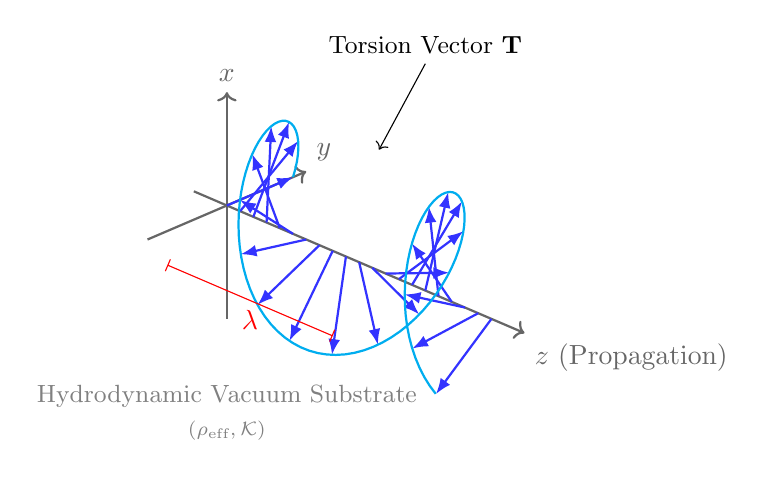
\begin{tikzpicture}[x={(0.7cm,-0.3cm)}, y={(0.7cm,0.3cm)}, z={(0cm,1cm)}, scale=1.2]

                        % --- Settings ---
                        \newcommand{\waveL}{4} % Length of wave
                        \newcommand{\freq}{2.5} % Frequency
                        \newcommand{\amp}{1.0}  % Amplitude

                        % --- Axis ---
                        \draw[->, thick, black!60] (-0.5,0,0) -- (\waveL+0.5,0,0) node[anchor=north west] {$z$ (Propagation)};
                        \draw[->, thick, black!60] (0,-1.2,0) -- (0,1.2,0) node[anchor=south west] {$y$};
                        \draw[->, thick, black!60] (0,0,-1.2) -- (0,0,1.2) node[anchor=south] {$x$};

                        % --- The Torsion Wave (Helical Vectors) ---
                        \foreach \z in {0,0.2,...,\waveL} {
                            % Calculate coordinates
                            \pgfmathsetmacro{\ang}{\z * \freq * 180 / 3.14159}
                            \pgfmathsetmacro{\cy}{\amp * cos(\ang)}
                            \pgfmathsetmacro{\cx}{\amp * sin(\ang)}

                            % Draw Torsion Vector (T)
                            \draw[->, thick, blue!80, -{Latex[length=2mm]}]
                            (\z,0,0) -- (\z, \cy, \cx);
                        }

                        % --- The Envelope Curve (The Helix) ---
                        \draw[thick, cyan, samples=100, domain=0:\waveL, variable=\t]
                        plot (\t, {\amp * cos(\t * \freq * 180 / 3.14159)}, {\amp * sin(\t * \freq * 180 / 3.14159)});

                        % --- Annotations ---
                        % Label the Torsion Vector
                        \draw[<-, thin, black] (1.5, {0.8}, {0.8}) -- (1.5, 1.5, 1.5) node[anchor=south] {\small Torsion Vector $\mathbf{T}$};

                        % Wavelength
                        \draw[|-|, thin, red] (0.6, -1.5, 0) -- (3.1, -1.5, 0) node[midway, below] {$\lambda$};

                        \node[anchor=north, gray, align=center] at (3, -3, 0) {\small Hydrodynamic Vacuum Substrate \\ \scriptsize ($\rho_{\text{eff}}, \mathcal{K}$)};
                    \end{tikzpicture}
                    \caption{\textbf{The Photon as a Propagating Torsional Shear Wave.} The electromagnetic field corresponds to a continuous transverse oscillation of the substrate's director field. The blue vectors trace a helical path, satisfying $\Box \mathbf{A} = 0$.}
                    \label{fig:torsion_wave}
            \end{figure}

            \subsection{The Hydrodynamic Lagrangian}
                The dynamics of the substrate are governed by an effective Lagrangian density $\mathcal{L}$ constructed from kinetic energy and elastic energy:
                \begin{equation}
                    \mathcal{L} = \frac{1}{2}\density \|\flow\|^2 - \frac{1}{2}\tension \|\nabla \times \pot\|^2.
                \end{equation}
                Identifying the speed of light as:
                \begin{equation}
                    c = \sqrt{\frac{\tension}{\density}},
                \end{equation}
                this becomes the Coulomb-gauge form of the gauge-invariant Maxwell action $S=-\frac{1}{4\mu_0}\!\int F_{\mu\nu}F^{\mu\nu}d^4x$ under the identifications $\varepsilon_0 \equiv \density$ and $1/\mu_0 \equiv \tension$.

            \subsection{Derivation of the Wave Equation}
                    Applying the Euler–Lagrange equations to $A_i$:
                    \begin{align}
                        \partial_t \Big(\frac{\partial \mathcal{L}}{\partial (\partial_t A_i)} \Big) &= \density \,\partial_t^2 A_i, \\
                        \nabla \cdot \Big(\frac{\partial \mathcal{L}}{\partial (\nabla A_i)} \Big) &= -\density \, c^2 [\nabla \times (\nabla \times \pot)]_i.
                    \end{align}

                Combining these yields the vector wave equation:
                \begin{equation}
                    \density (\partial_t^2 \pot + c^2 \nabla \times \nabla \times \pot) = 0.
                \end{equation}
                Using the vector identity $\nabla \times \nabla \times \pot = \nabla(\nabla \cdot \pot) - \nabla^2 \pot$ and $\nabla \cdot \pot = 0$, we recover the exact massless wave equation:
                \begin{equation}
                    \boxed{ \Box \pot = \left( \frac{1}{c^2}\partial_t^2 - \nabla^2 \right) \pot = 0 }.
                \end{equation}

                This derivation demonstrates that Maxwell's equations for the photon emerge naturally from the mechanics of an incompressible, elastic fluid substrate, without postulating the field as a fundamental entity.

        \section{Prediction: Vacuum Faraday Rotation}\label{sec:prediction}
            A key consequence of this framework is that the vacuum behaves as a magneto-optical medium. In the presence of a parity-odd substrate coupling (background vorticity), the vacuum exhibits intrinsic birefringence.

            \subsection{Swirl-Induced Birefringence}
                Consider a photon (transverse shear wave) with frequency $\omega_\gamma$ and wavevector $\mathbf{k}$ propagating through a background fluid substrate rotating with vorticity $\vorticity$. In the rotating frame, the wave equation is modified by the Coriolis acceleration term $2\vorticity \times \partial_t \pot$.

                This leads to a modified dispersion relation for the Left ($L$) and Right ($R$) chiral modes:
                \begin{equation}
                    \omega^2 \approx c^2 k^2 \pm 2 \omega \vorticity \cdot \hat{k}.
                \end{equation}
                Solving for the refractive index $n = ck/\omega$, we obtain the splitting:
                \begin{equation}
                    n_{L/R} \approx 1 \pm \frac{\vorticity \cdot \hat{k}}{\omega_{\gamma}}.
                \end{equation}
                This difference in phase velocity induces a rotation of the polarization plane (Faraday Rotation) by an angle $\Delta \theta$ over a propagation distance $L$:
                \begin{equation}
                    \Delta \theta = \frac{\omega_\gamma L}{2c} (n_L - n_R) \approx \frac{L}{c} (\vorticity \cdot \hat{k}).
                \end{equation}

            \subsection{The Vacuum Verdet Constant}
                To formalize this in a gauge-invariant effective field theory, we introduce the Carroll–Field–Jackiw (CFJ) term:
                \begin{equation}
                    S_{\text{odd}} = \frac{1}{2}\!\int\! p_\mu \,\epsilon^{\mu\nu\rho\sigma} A_\nu F_{\rho\sigma}\, d^4x,
                \end{equation}
                where the axial vector $p_\mu$ is determined by the substrate background. Mapping the hydrodynamic vorticity to the magnetic field ($p_\parallel = \alpha_{\text{vac}} \Bbg \cdot \hat{k}$), we derive the  \textbf{Vacuum Verdet Constant}:
                \begin{equation}
                    \boxed{\, \mathcal{V}_{\text{vac}} \equiv \frac{\theta}{B\,L} \approx \frac{\alpha_{\text{vac}}}{2} \,}\,.
                \end{equation}
                This predicts \emph{linear-in-$B$} Faraday rotation in vacuum, distinct from the parity-even, quadratic-in-$B$ birefringence ($\Delta n \propto B^2$) predicted by standard QED (Euler-Heisenberg).

            \subsection{Detectability and Regimes}
                The observation of this effect depends on overcoming the suppression by the microscopic scale $\microlength$. Two promising regimes are:
                \begin{enumerate}
                    \item \textbf{Extreme Path Lengths:} In cosmological or astrophysical baselines, the integrated rotation $\theta \sim \mathcal{V}_{\text{vac}} \int B_\parallel dl$ may become detectable. Crucially, this geometric rotation is  \textbf{wavelength-independent}, distinguishing it from the plasma Rotation Measure (RM) which scales as $\lambda^2$.
                    \item \textbf{Ultra-Strong Fields:} Environments like Magnetars ($B \sim 10^{10-11}$ T) and high-intensity laser setups (ELI-NP, LUXE) maximize $B_\parallel$. In these regimes, the linear scaling ($\theta \propto B$) of the hydrodynamic vacuum effect can be separated from the quadratic ($\theta \propto B^2$) QED effect.
                \end{enumerate}

                Current laboratory constraints (e.g., PVLAS~\cite{bregant2008}) place upper bounds on $\alpha_{\text{vac}}$. A non-null detection of linear vacuum rotation in future experiments would serve as direct evidence for the hydrodynamic substrate.

            \subsection{Comparison with QED}
                Standard Quantum Electrodynamics (QED) predicts a vacuum birefringence due to the Euler–Heisenberg Lagrangian:
                \begin{equation}
                    \Delta n_{\text{QED}} \propto B^2.
                \end{equation}
                Crucially, pure-vacuum QED is parity even: it yields \emph{no Faraday rotation} (no linear-in-$B$ term). In contrast, our hydrodynamic model predicts a birefringence that is \textbf{linear} in $B$ (geometric). This distinct scaling behavior provides a clear ``smoking gun'' for experimental verification.

        \section{Experimental Implications}\label{sec:experiments}
            We propose several experimental avenues to test this hydrodynamic theory of light.

            \subsection{Optical Vortex Beams}
                High-order Laguerre–Gaussian (LG) beams carry orbital angular momentum (OAM). In our framework, high-OAM beams mimic the vorticity structure of the substrate. We predict anomalous group delays for these beams in rotating media or materials with strong spin–orbit coupling.

            \subsection{Superfluid Analogs}
                Bose–Einstein condensates and superfluid helium act as laboratory analogs. Rotating toroidal traps could display chiral splitting of phonon analogs, mirroring the substrate-induced parity-odd response.

            \subsection{Vacuum Birefringence Tests}
                Future high-intensity laser experiments (ELI-NP, LUXE) and observations of magnetars can probe vacuum optical properties. A deviation from the $B^2$-only scaling would support the torsion-projection hypothesis.

        \section{Conclusion}\label{sec:conclusion}
            We presented a geometric unification of electromagnetism and fluid dynamics. Identifying $F$ as a projection of Cartan torsion in a teleparallel, director-bearing substrate recovers the Maxwell wave equation in a gauge-fixed hydrodynamic representation with $c=\sqrt{\tension/\density}$.

            A common objection to hydrodynamic vacuum models is the apparent violation of Lorentz invariance. However, as demonstrated in analogue gravity literature,  \textbf{Lorentz invariance naturally emerges as an approximate acoustic symmetry} of the fluid equations in the low-energy limit~\cite{barcelo2011}. Thus, this framework remains consistent with relativistic observations at standard energy scales.

            Most importantly, this framework predicts a non-zero Vacuum Verdet constant ($\mathcal{V} \sim \alpha_{\text{vac}}/2$). While current experiments constrain this effect, it remains a falsifiable prediction distinguishable from the quadratic $B^2$ scaling of QED vacuum polarization. Future work will explore how topological defects in this substrate—knotted vortices—may give rise to massive fermions, aligning this framework with emerging vortex-string models of particle physics.

            \section*{Author Contributions Statement}
            \textbf{Omar Iskandarani:} Conceptualization, Methodology, Formal Analysis, Investigation, Writing -- Original Draft, and Writing -- Review \& Editing. The author confirms sole responsibility for the following study conception and design, data collection, analysis and interpretation of results, and manuscript preparation.

        \bibliographystyle{unsrt}
        \begin{thebibliography}{99}
            \bibitem{helmholtz1858} H. von Helmholtz, \textit{On Integrals of the Hydrodynamical Equations which Express Vortex Motion}, J. Reine Angew. Math. \textbf{55}, 25 (1858).
            \bibitem{kelvin1867} W. Thomson (Lord Kelvin), \textit{On Vortex Atoms}, Proc. R. Soc. Edin. \textbf{6}, 94 (1867).
            \bibitem{maxwell1875} J. C. Maxwell, \textit{A Treatise on Electricity and Magnetism}, Clarendon Press, Oxford (1875).
            \bibitem{unruh1981} W. G. Unruh, \textit{Experimental Black-Hole Evaporation?}, Phys. Rev. Lett. \textbf{46}, 1351 (1981).
            \bibitem{volovik2003} G. E. Volovik, \textit{The Universe in a Helium Droplet}, Oxford Univ. Press (2003).
            \bibitem{barcelo2011} C. Barceló, S. Liberati, and M. Visser, \textit{Analogue Gravity}, Living Rev. Relativ. \textbf{14}, 3 (2011).
            \bibitem{kobayashi2025} S. Kobayashi et al., \textit{Revisiting Volterra defects}, R. Soc. Open Sci. \textbf{12}, 242213 (2025).
            \bibitem{heisenberg1936} W. Heisenberg and H. Euler, \textit{Consequences of Dirac's Theory}, Z. Phys. \textbf{98}, 714 (1936).
            \bibitem{fedi2023} M. Fedi, \textit{Gravity as a Fluid Dynamic Phenomenon}, Zenodo (2023).
            \bibitem{bregant2008} M. Bregant et al. (PVLAS), \textit{Limits on Low-Energy Photon-Photon Scattering}, Phys. Rev. D \textbf{78}, 032006 (2008).
        \end{thebibliography}

\end{document}